\documentclass[a4paper]{article}
\usepackage[T1]{fontenc}
\usepackage{amsmath}
\usepackage{amsthm}
\usepackage{amssymb}
\usepackage{float}
\usepackage[utf8]{inputenc}
\usepackage{graphicx}
\usepackage[italian]{babel}
\usepackage{thmtools}
\newtheorem{theorem}{Theorem}
\newtheorem*{definition}{Definizione}
\newtheorem{example}{Example}

\begin{document}

\author{Lorenzo Dentis, lorenzo.dentis@edu.unito.it}
\title{Esercizio 1}
\maketitle

\section{logica proposizionale}
\subsection{Esercizio 1}
Which of the following propositional formulas represents the sentence, 'He will come on the 8:15 or the 9:15 train; if the former, he will have time to visit us', where
\begin{itemize}
	\item p means 'He will come on the 8:15'
	\item q means 'He will come on the 9:15'
	\item r means 'He will have time to visit us'
\end {itemize}
Risposta 5: $(p \lor  q) \land (p \rightarrow r)$
\subsection{Esercizio 2}
Which of the following sentences has the logical form $(p \land q) \rightarrow r$ ?\\
Risposta 3: If inflation is up and an election is approaching, then public borrowing goes up.
\subsection{Esercizio 3}
Which of the following propositional formulas is satisfied by the valuation which assigns T to P, and F to q and r.\\
Risposta 2: $\lnot ( \lnot r \rightarrow ( p \land q))$
\subsection{Esercizio 4}
Which of the following propositional formulas is a tautology?\\
Risposta 5: $ (p \leftrightarrow q) \land (p \leftrightarrow \lnot q)$
\subsection{Esercizio 5}
Which of the following entailments is valid?\\
Risposta 2: $ p, \lnot p \leftrightarrow q \models \lnot q $
\subsection{Esercizio 6}
Risposta 3:
\begin{displaymath}
\begin{array}{|c c c|c|}
p & q & r & (p \rightarrow q) \lor \lnot (r \land \lnot q) \\
\hline 
T & T & T & T \\
T & T & F & T \\
T & F & T & F \\
T & F & F & T \\
F & T & T & T \\
F & T & F & T \\
F & F & T & T \\
F & F & F & T \\
\end{array}
\end{displaymath}
\subsection{Esercizio 7}
Which of the following formulas represents the sentence 'If Smith has installed central heating, then he has sold his car or he has not paid his mortage', where:
\begin{itemize}
	\item p means 'Smith has installed central heating'
	\item q means 'Smith has sold his car'
	\item r means 'Smith has paid his mortage'.
\end{itemize}
Risposta 4: $ p \rightarrow q \lor \not r $
\subsection{Esercizio 8}
Which of the following formulas represents the sentence, 'Share prices will go up, and if interest rates go up too, there will be a recession', where:
\begin{itemize}
	\item p means 'share prices will go up'
	\item q means 'interest rates will go up'
	\item r means 'there will be a recession'.
\end{itemize}
Risposta 2: $p \land (q \rightarrow r) $
\subsection{Esercizio 9}
Which of the following sentences could be written as $ p \lor (q \land r)$, for suitable p, q, and r ?\\
Risposta 2 : You can go swimming, or use the sauna and the shower.
\subsection{Esercizio 10}
According to the standard convention about binding priorites, the formula, $ \lnot p \rightarrow \lnot q \land r $, is implicity one of the following. Which?\\
Risposta 4: $ ( \lnot p) \rightarrow (( \lnot q) \land r) $
\subsection{Esercizio 11}
Which of the following formulas has the parse tree:\\
\begin{figure}[H]
	\centering
	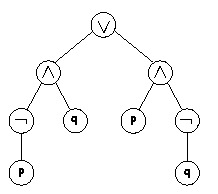
\includegraphics[scale = 0.5]{parsetree.jpg}
\end{figure}
Risposta 1: $ ( \lnot p \land q) \lor (p \land \lnot q) $

\section{notazioni e definizioni}
\subsubsection{Insiemi}
notazione per Naturali $ \mathbb{N} $, Interi $ \mathbb{Z} $, Reali $ \mathbb{R} $,\\ elemento contenuto in un insieme $ \in $
\newline
\begin{definition}[Intersezione]L'intersezione ($\cap$) tra due insiemi $A$ e $B$ è l'insieme degli elementi che appartengono contemporaneamente sia ad $A$ che a $B$\\ 
	\begin{center}$A \cap B = \{x:x \in A \: and \: x \in B\}$\end{center}
\end{definition}
\begin{definition}[Unione]L'unione $\cup$ tra due insiemi $A$ e $B$ è l'insieme degli elementi che appartengono ad $A$, a $B$ o ad entrambi.
	\begin{center}$A \cup B = \{x:x \in A \: or \: x \in B\}$\end{center}
\end{definition}
\begin{definition}[Differenza]La differenza $\setminus$ tra due insiemi $A$ e $B$, indicata con $A \setminus B$ è l'isieme degli elementi di $A$ esclusi gli elementi che appartengono anche a $B$
	\begin{center}$A \setminus B = \{x:x \in A \: and \: x \in B\}$\end{center}
\end{definition}
\begin{definition}[Power Set]L' insieme potenza (power set) $\mathcal{P}$($A$) è l'insieme di tutti i sottoinsiemi di $A$, compreso l'insieme vuoto $\emptyset$ e l'insieme $A$ stesso.\begin{center} $\mathcal{P}(A)=\{X : X \subseteq A\}$ \end{center}
\end{definition}
\begin{definition}[Complemento]L'insieme complemento di un inseme $A$, scritto $A^{C}$, è l'insieme ottenuto dalla differenza tra l'insieme Universo ed $A$.\begin{center} $A^{C} = U \setminus A$\end{center}
\end{definition}
\begin{definition}[Sottoinsieme]Un sottinsieme $ \subseteq $  di $A$ è un insieme che contiene solamente gli elementi contenuti in $A$, eventualmente tutti.
$$ X \subseteq A \Leftrightarrow X = \{x \vert x \in A \}$$
\end{definition}
\begin{definition}[Sottoinsieme stretto]
Un sottinsieme stretto $ \subset $ di $A$ è un insieme che contiene solamente elementi contenuti in $A$, ma non tutti.
$$ X \subset A \Leftrightarrow X = \{x \vert x \in A \} \land X \neq A$$
\end{definition}

\subsubsection{relazioni}
\begin{definition}[Prodotto Cartesiano]Il prodotto cartesiano di due insiemi $A$ e $B$ è l'insieme delle coppie ordinate $(a,b)$ con $a \in A$ e $b \in B$ Formalmente:\begin{center}
$A\times B:=\{(a,b):a\in A\;{\mathrm  {e}}\;b\in B\}$\end{center}
\end{definition}
\begin{definition}[Relazione binaria]
Si definisce relazione binaria $R$ tra due insiemi non vuoti $A$ e $B$ un sottoinsieme di $ A \times B$. Due elementi $x$ e $y$ sono messi in relazione da $R$ se: 
$(x,y)\in R\ $ ed in tal caso si scrive $xRy$.
\end{definition}
\begin{definition}[Relazione riflessiva]
Una relazione binaria $R$ in un insieme $X$ è detta riflessiva se ogni elemento di $X$ è in tale relazione con sé stesso.
\begin{center} $R$ è riflessiva se: $ \forall a\in X,\ aRa.$ \end{center}
\end{definition}
\begin{definition}[Relazione simmetrica]Una relazione binaria $R$ in un insieme$ X $è simmetrica se e solo se, presi due elementi qualsiasi $a$ e $b$, vale che se $a$ è in relazione con $b$ allora anche $b$ è in relazione con $a$.\\
\begin{center}$\forall a,b\in X,\ aRb\Rightarrow bRa$\end{center}
\end{definition}
\begin{definition}[Relazione transitiva]Una relazione transitiva $R$ in un insieme $X$ è transitiva se e solo se prendendo tre elementi qualsiasi $a$, $b$ e $c$ $ \in X$, tali che $aRb$ e $bRc$ allora $aRc$
	$$\forall a,b,c \in X,aRb \wedge bRc \Rightarrow aRc$$
\end{definition}
\begin{definition}[Relazione di equivalenza]Una relazione di equivalenza $R$ su $A$ è una relazione riflessiva, simmetrica e transitiva.
\end{definition}
\begin{definition}[Chiusura transitiva di una relazione]Data una relazione $R$ su $A\times A$ chiamiamo chiusura transitiva di $R$, e la indichiamo con $R^{+}$ la seguente relazione:
\begin{center}$ R^{+} = \{ x, y | \exists z_1,.....,z_n \in A, n \geq 2, z_1 = x, z_n = y$ t.c $ y_iRy_{i+1}$ con $ i=1,....,n-1 \} $ \end{center}
\end{definition}
\begin{definition}[Funzione]Una funzione è una relazione tra due insiemi che associa ad ogni elemento di $A$ uno ed un solo elemento di $B$
\begin{center}$\forall a \in A \ \ \exists  ! \ b \in B \ \mbox{ tale che } \ f:a\to b$\end{center}
\end{definition}
\begin{definition}[Funzione  di arietà n]L'arietà di una funzione è il numero di argomenti che la funzione richiede. posta una funzione $f : A^{n} \rightarrow A$ la sua arietà è $n$ 
\end{definition}
\begin{definition}[Funzione iniettiva]Una funzione $f : A \rightarrow B $è iniettiva se ad ogni elemento $a$ del dominio $A$ corrisponde attraverso $f$ al più un elemento $b$ del codominio $B$.
	\begin{center}$\forall a\in A\ \ \exists! b\in B \mbox{ t.c. }f(a)=b$\end{center}
\end{definition}
\begin{definition}[Funzione suriettiva]Una funzione $f : A \rightarrow B $è suriettiva se ogni elemento $b$ del codominio $B$ è immagine di almeno un elemento $a$ del dominio $A$.
	\begin{center}$\forall b\in B\ \ \exists a\in A\ \mbox{ t.c. }f(a)=b$\end{center}
\end{definition}
\begin{definition}[Funzione biiettiva]Una funzione $f$ che è contemporaneamente iniettiva e suriettiva.
\end{definition}

\subsubsection{Stringhe e linguaggi}

\begin{definition}[Alfabeto]Alfabeto $\Sigma$: insieme non vuoto e finito di simboli.
\end{definition}

\begin{definition}[Lettera e stringa]Posto un alfabeto $\Sigma$, una lettera è un elemento $\in \Sigma$, una stringa è una sequenza ordinata e finita di lettere.
\end{definition}

\begin{definition}[String vuota]Stringa di lunghezza 0, si indica con $\epsilon$, la si può anche definire come l' elemento neutro rispetto all'operazione concatenazione $\cdot$
\end{definition}

\begin{definition}[Concatenazione] Il concatenamento di due stringe $L_1$,$L_2$, indicato con "$\cdot$" o semplicemente senza alcun carattere, da origine alla stringa $L_1L_2$ di lunghezza $|L_1| + |L_2|$ che presenta ordinatamente i caratteri di $L_1$ seguiti da quelli di $L_2$.
\end{definition}

\begin{definition}[Prefisso e Suffisso]Data una stringa $S = t_1,$...,$t_n$ definiamo prefisso la stringa $S^1 = t_1,$...,$t_m$ con $ 0 < m < n$. Invece definiamo suffisso la stringa $S^2 = t_m,$...,$t_n$ con $ 0 < m < n$ 
\end{definition}


\subsubsection{Grafi}

Per tutte le seguenti definizioni poniamo un grafo $G =(V, E)$, ove $V$ è l'insieme dei nodi (Vertex)ed $E$ l'insieme degli archi (Edges). In particolare $E \subseteq V\times V$  
\begin{definition}[Direzione]Identifichiamo con $R$ la relazione che indica due nodi $a$,$b$$\in V$ connessi tra loro da un arco, diciamo che il grafo è non-orientato se $R$ è simmetrica, orientato altrimenti.
\end{definition}

\begin{definition}[Grafo bipartito]Un grafo si dice bipartito quando l'insieme $V$ può essere bipartito in due sottoinsiemi disgiunti $V=V_1\cup V_2$ tali che ogni arco $\{v_1,v_2\} \in E$ rispetta la seguente forma: $v_1 \in V_1 \land v_2 \in V_2$
\end{definition}

\begin{definition}[nodo sorgente/destinazione]Un nodo $v \in V$ è detto nodo sorgente se non ha archi entranti, nodo destinazione se non ha archi uscenti.\\
In simboli: posta la relazione $R$ per cui $v_1Rv_2$ indica un arco diretto da $v_1 a v_2$ un nodo sorgente è $v t.c. \forall {v,u} \in E vRu$\\
Un nodo destiazione è $v t.c. \forall {v,u} \in E uRv$
\end{definition}

\begin{definition}[in-degree, out-degree]Il grado (Degree) di un nodo $v \in V$ è il numero di archi $e = \{v,v_x\}\in E$, cioè il numero di archi connessi al nodo.\\
Usando la relazione $R$ della precendente definizione: out-degree di $v$ è il numero di archi ${v,u} t.c. vRu$, in-degree di $v$ è il numero di archi ${v,u} t.c. uRv$
\end{definition}

\begin{definition}[Funzione di etichettatura]Una funzione che attribuisce un valore numerico ad ogni nodo.\\
Più formalmente un'etichettatura di vertice è una funzione $f: V \rightarrow \mathbb{N}$ 
\end{definition}

\begin{definition}[Cammino]Una n-upla di nodi $(v_0, ..., v_m)$ è un cammino quando: $(\forall i=1,...,m)(v_{i-1},v_{i})\in E$ con $v_0 \neq v_m$
\end{definition}

\begin{definition}[Ciclo]Una n-upla di nodi $(v_0, ..., v_m)$ è un cammino quando: $(\forall i=1,...,m)(v_{i-1},v_{i})\in E$ con $v_0 = v_m$
\end{definition}

\begin{definition}[Lunghezza di un cammino]Sia un cammino n-upla di nodi $c=(v_0, ..., v_m)$, la lunghezza del cammino $|c|$ è il numero di nodi $\in c$
\end{definition}

\begin{definition}[Grafo fortemente connesso]Un grafo orientato si dice fortemente connesso se esiste un cammino da $v$ a $u$ per ogni coppia $v,u \in V$
\end{definition}

\begin{definition}[Componente fortemente connessa terminale]Una componente fortemente connessa di un grafo diretto G è un sottografo di G in cui esiste un cammino orientato tra ogni coppia di nodi ad esso appartenenti.La componente fortemente connessa terminale è la componente fortemente connessa massimale, quella che contiene più nodi possibili
\end{definition}

\begin{definition}[Albero]Un albero è un grafo connesso ed aciclico, più precisamente un grafo non orientato nel quale due vertici qualsiasi sono connessi da un solo cammino.


\end{definition}

\subsubsection{Matrici}

\begin{definition}[Matrici n-dimensionali]una matrice è una funzione $ A\colon X_1 \times X_2 \times ... \times X_n \rightarrow K $ ove n è il numero di dimensioni della matrice.
\end{definition}

\begin{definition}[Somma di matrici]Date due matrici $A$ e $B$, entrambe di tipo $m \times n$, $A + B$ è una matrice $m \times n$ i cui elementi sono $[A+B]_{i,j}:=[A]_{i,j}+[B]_{i,j}$
\end{definition}

\begin{definition}[Prodotto di matrici]Date due matrici $A$ e $B$ rispettivamente di tipo $m \times p$ e $p \times n$, il prodotto è una matrici di tipo $m \times n$ i cui elementi sono: $[C]_{i,j}=Row_{i}(A)\times Col_{j}(B)=[A]_{i,1}[B]_{1,j}+[A]_{i,2}[B]_{2,j}+\cdots +[A]_{i,p}[B]_{p,j}$
\end{definition}

\begin{definition}[Vettore per matrice]Il prodotto di un vettore $V$, con $|V| = m$, per una matrice $M$ di tipo $m \times n$ è un vettore $V \times M$ di lunghezza $m$ i cui elementi sono: $[C]_{i}=[V]_{i} B[i,2] + [V]_{i} B[i,2] + ..... + [V]_{m} B[m,n]$
\end{definition}


\end{document}
